\documentclass[11pt]{article}
\usepackage{hyperref} 
\usepackage{amsmath, amsfonts, amssymb}
\usepackage{graphicx}
\usepackage{float}
\usepackage[margin=1in]{geometry}

\parindent0px

\emergencystretch=0pt
\pretolerance=150
\tolerance=10000
\hbadness=10000
\hfuzz=0pt

\title{Introduction to Linear Algebra Notes}
\author{Nathan Ueda}
\date{\today} 

\begin{document}
\maketitle 
\pagebreak
\tableofcontents 
\pagebreak

\section{Vectors and Matrices}
\subsection{Vectors and Linear Combinations}

\textbf{Vector Length:} For a vector $ v \in \mathbb{R}^n $, its length is:

\[ \|v\|= \sqrt{v_1^2 + \cdots + v_n^2} \]

In words, the length of a vector is the square root of the sum of the squared components. \\

Given two vectors in $\mathbb{R}^2\ v, w$ with their tail starting from the origin
\begin{itemize}
    \item If they lie on the same line, the vectors are \textit{linearly dependent}.
    \item If they do not lie on the same line, the vectors are \textit{linearly independent}.
\end{itemize}
Therefore, the combinations $ c\textbf{v} + d\textbf{w} $ fill the $x-y$ plane unless $v$ is in 
line with $w$. \\

To fill $m$-dimensional space, we need $m$ independent vectors, with each vector having $m$
components.

\subsection{Lengths and Angles from Dot Products}

\textbf{Dot Product:} For two vectors $v, w \in \mathbb{R}^n$, their dot product is:

\[ v \cdot w = v_1 w_1 + \cdots + v_n w_n \]

The dot product of two vectors tells us what amount of one vector goes in the direction of
another. It tells us how much these vectors are working together.

\begin{itemize}
    \item $ v \cdot w > 0 $: The vectors point in somewhat similar directions. In other
    words, the angle between the two vectors is less than 90 degrees.
    \item $ v \cdot w = 0 $: The vectors are perpendicular. In other words, the angle 
    between the two vectors is 90 degrees.
    \item $ v \cdot w < 0 $: The vectors point in somewhat opposing directions. In other
    words, the angle between the two vectors is greater than 90 degrees.
\end{itemize}

Dot Product Rules (for two vectors, v, w):
\begin{itemize}
    \item $ v \cdot w = w \cdot v $
    \item $ u \cdot (v + w) = u \cdot v + u \cdot w $
    \item $ (cv) \cdot w = c(v \cdot w) $
\end{itemize}

\textbf{Cosine Formula:} If $v$ and $w$ are nonzero vectors, then:
\[ \cos \theta = \frac{v \cdot w}{\|v\| \|w\|}\]

\textbf{Unit Vectors:} A vector is a unit vector if its length is 1. \\
For a vector $u \in \mathbb{R}^n$:

\[ \|u\| = 1\]

For any vector $v \in \mathbb{R}^n$, as long as $v \ne 0$, dividing $v$ by its length will
result in a unit vector. In other words:

\[ u = \frac{v}{\|v\|} \]

\textbf{Cauchy-Schwarz Inequality:} 
\[ | v \cdot w | \le \|v\|  \|w\| \]
In words, the absolute value of the dot product of two vectors is no greater than the product 
of their lengths.

\textbf{Triangle Inequality:} 
\[\|v + w\| \le \|v\| + \|w\|\]
In words, the length of any one side (in this case $\|v+w\|$) of a triangle is at most the sum
of the length of the other triangle sides.

\begin{figure}[H] 
	\centering 
	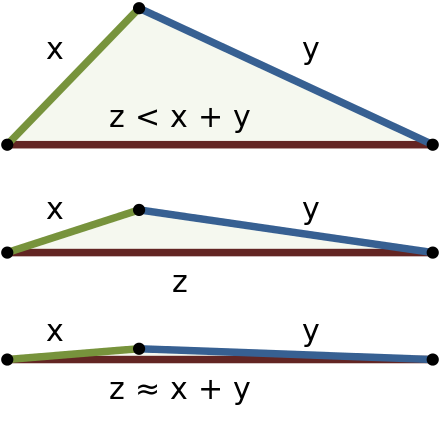
\includegraphics[width=2in]{imgs/triangle_inequality.png}
	\caption{This Squeeze Theorem}
\end{figure}

\end{document}